\chapter{Étude et réalisation du Sprint 1}
\section{Introduction}
\noindent
Après avoir examiné l'étude technique de notre projet d'assurance automobile en ligne, nous entamons maintenant le Sprint 1, qui ce concentra sur la création d'un systéme de recherche des produits dans la langue Française.

\section{Backlog du Sprint 1}
\noindent
Le backlog de notre premier Sprint est présenté dans le tableau ~\ref{tab:sprint1}.

\begin{table}[H]
	\centering

	\begin{tabularx}{\textwidth}{|c|X|c|c|}
		\hline
		\rowcolor{blue!20}
		\textbf{ID} & \textbf{Scénario}                                                                                     & \textbf{Priorité} & \textbf{Complexité} \\ \hline
		1           & En tant qu'un client, je veux saisir ma terme de recherche en Français pour chercher le(s) produit(s) & 1                 & 10                  \\ \hline
	\end{tabularx}
	\caption{Backlog du Sprint 1}
	\label{tab:sprint1}
\end{table}

\section{Spécification fonctionnelle}
\noindent
Dans cette partie, on va expliquer les différentes fonctionnelités du Sprint 1 à travers le diagramme de cas d'utilisation. Puis en va exposer les différents scénarios de notre cas d'utilisation à travers des descriptions textuelles.

\subsection{Diagramme de cas d'utilisation général}
\begin{figure}[H]
	\centering
	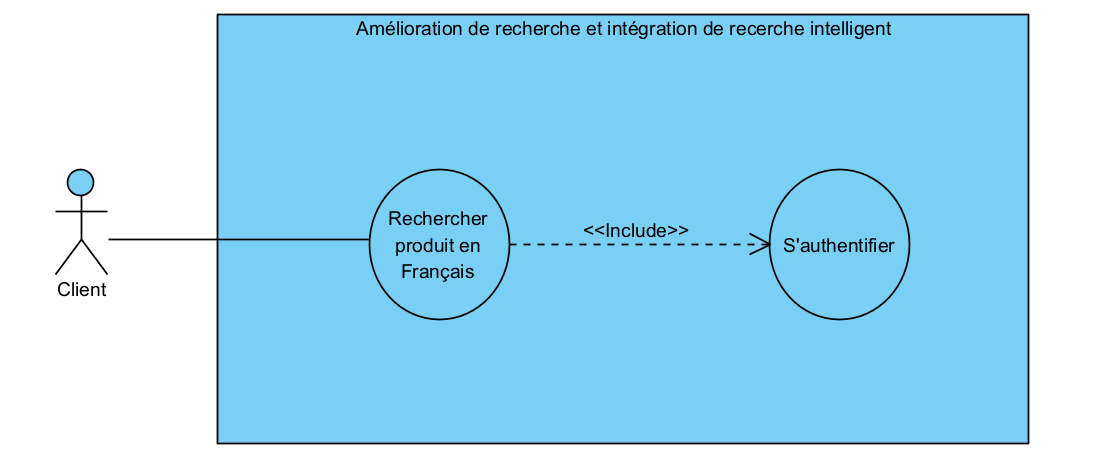
\includegraphics[width=1\textwidth]{logos/recherchefrancais.png}
	\caption{Diagramme de cas d'utilisation général du Sprint 1}
	\label{fig:recherchefrancais}
\end{figure}

\subsection{Description textuelle du CU << Rechercher produit en Français >>}
\noindent
\textbf{Titre:} Rechercher produit en Français \\
\textbf{Résumé:} Le client saisit son terme de recherche (en Français), en cliquant sur la boutton pour rechercher le(s) produit(s) qu'il veut chercher. \\
\textbf{Acteur Principal:} Client \\
\textbf{Précondition:} Le client est authentifié \\
\textbf{Postcondition:} Le(s) produit(s) que le client cherche est renvoyé, si'il n'existe pas, le systéme renvoie des produits similaires comme suggestion. \\
\textbf{Scénario de base: }
\begin{enumerate}
	\item Le client saisit son terme de recherche.
	\item Le client clique sur la boutton "Rechercher"
	\item Le systéme prend cette terme de recherche, et performe les étapes nécessaires pour la convertir en vecteur.
	\item Le systéme compare cette vecteur contre les vecteurs dans Elasticsearch.
	\item Le systéme renvoie les produits.
\end{enumerate}

\newpage
\textbf{Scénario alternatifs : }
\begin{enumerate}
	\item La terme de recherche est vide:
	      \begin{enumerate}
		      \item Le système affiche un message d'erreur informant le client que la terme de recherche est requis.
		      \item Retour à l'étape 1 du scénario de base.
	      \end{enumerate}

	\item Le(s) produit(s) que le client cherche n'existe pas.
	      \begin{enumerate}
		      \item Le systéme essaie de renvoyer les produits les plus similaires comme des suggestions.
		      \item Retour à l'étape 1 du scénario de base.
	      \end{enumerate}
\end{enumerate}

\subsection{Diagramme de séquence detaillé}
\noindent
En adoptant l'architecture MVC dans le chapitre précédent, nous avons choisi de
suivre ce modèle pour simplifier la création des diagrammes de séquence. Cette section
présentera le diagramme de séquence de cas d'utilisation << Rechercher produits en Français >> qui est présenté dans la figure ~\ref{fig:seqrecherchefrancais}.

\begin{figure}[H]
	\centering
	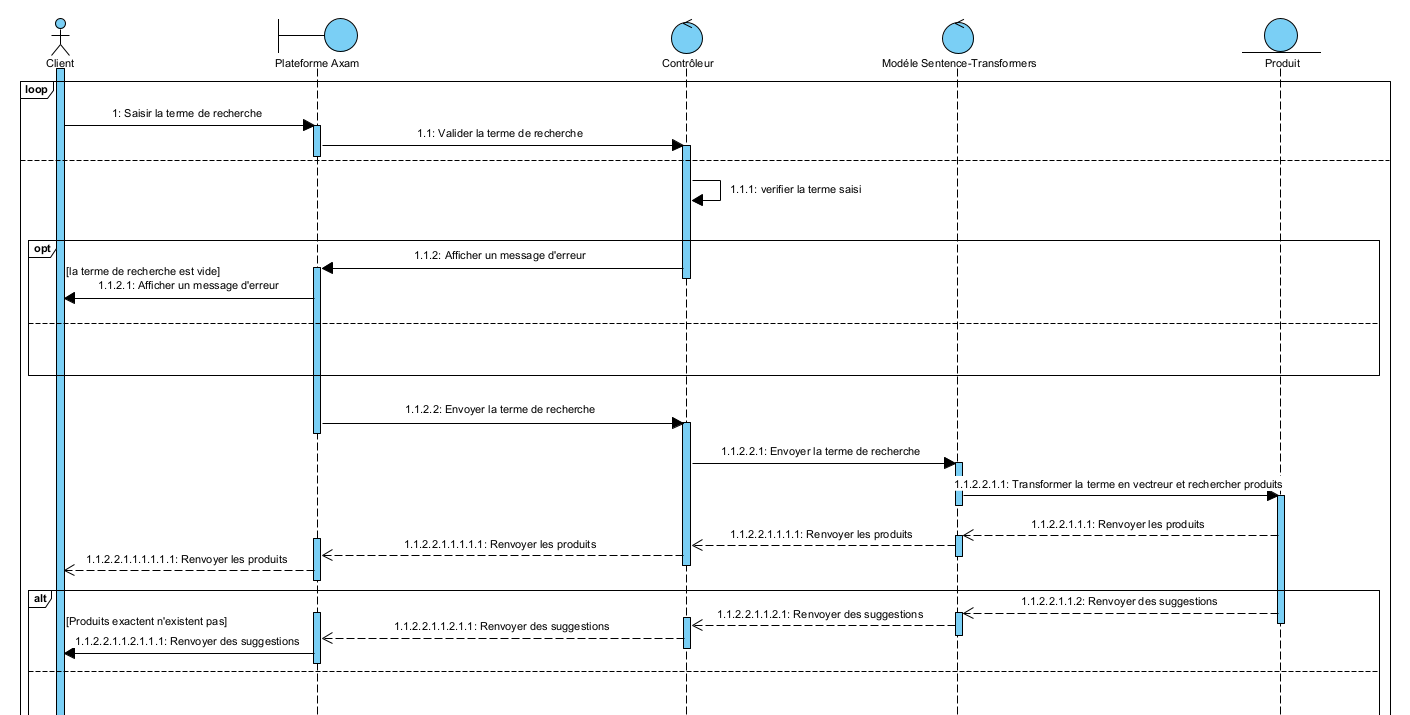
\includegraphics[width=1\textwidth]{logos/sequencerecherchefrancais.png}
	\caption{Diagramme de séquence de cas d’utilisation « Rechercher produits en Français »}
	\label{fig:seqrecherchefrancais}
\end{figure}

\section{Architecture de la base de données}
\noindent
Dans le cadre de notre projet, l'intégration d'Elasticsearch et MySQL génére un ensemble de tables indispnesables pour garantir son fonctionnement interne. Cependant, nous avons décidé de mettre l'accent uniquement sur les tables
spécifiques à notre projet durant la conception.

\subsection{Diagramme de classes}

\subsection{Schéma de la base de données}
\noindent
Suite à l'exploration du modèle conceptuel de la base de données pour le premier
sprint, nous allons maintenant décrire sa transposition en modèle logique, illustré par les tables dans les sections suivantes.

\subsection{Tables de base de données MySQL}
\begin{table}[H]
	\centering
	\Large
	\rowcolors{2}{white}{white} % To reset alternate colors if previously set
	\begin{tabular}{|p{4cm}|p{4cm}|p{4cm}|}
		\hline
		\rowcolor{blue!50} \textcolor{white}{Champs} & \textcolor{white}{Type} & \textcolor{white}{Contrainte} \\
		\hline
		id                                  & Auto-incrément          & Clé primaire                  \\ \hline
		email                                          & String                  & Non nul                       \\ \hline
		password                          & String                    & Non nul                       \\ \hline
		role                                   & String                  & Non nul                       \\ \hline
	\end{tabular}
	\caption{Table Client}
	\label{tab:table_client}
\end{table}

\begin{table}[H]
	\centering
	\Large
	\rowcolors{2}{white}{white} % To reset alternate colors if previously set
	\begin{tabular}{|p{4cm}|p{4cm}|p{4cm}|}
		\hline
		\rowcolor{blue!50} \textcolor{white}{Champs} & \textcolor{white}{Type} & \textcolor{white}{Contrainte} \\
		\hline
		id                                  & Auto-incrément          & Clé primaire                  \\ \hline
		word                                          & String                  & Non nul                       \\ \hline
		count                          & Int                    & Non nul                       \\ \hline
	\end{tabular}
	\caption{Table Keyword}
	\label{tab:table_keyword}
\end{table}

\subsection{Tables de base de données Elasticsearch}
\begin{longtable}{|l|l|p{5cm}|}
\caption{Table Produit} \label{tab:produit_table} \\
\hline
\rowcolor{blue!50} \textcolor{white}{Champs} & \textcolor{white}{Type} & \textcolor{white}{Contrainte} \\
\hline
\endfirsthead

\multicolumn{3}{c}%
{{\bfseries \tablename\ \thetable{} -- Suivie de la page précédente}} \\
\hline
\rowcolor{blue!50} \textcolor{white}{Champs} & \textcolor{white}{Type} & \textcolor{white}{Contrainte} \\
\hline
\endhead

% \hline \multicolumn{3}{|r|}{{Suivie sur la page suivante}} \\ \hline
% \endfoot

\hline
code interne & keyword &  \\ \hline
image produit & keyword &  \\ \hline
code a barre & keyword &  \\  \hline
REFERENCE & keyword &  \\ \hline
SKU & keyword &  \\ \hline
label produit & text &  \\ \hline
SEO label produit & text &  \\ \hline
categorie & keyword &  \\ \hline
sous-categorie & keyword &  \\ \hline
sous-sous-categorie & keyword &  \\ \hline
categorie\_id & integer &  \\ \hline
collection & text &  \\ \hline
Brève description & text &  \\ \hline
Description & text &  \\ \hline
Tags & text &  \\ \hline
fiche technique & text &  \\ \hline
alt image(71 caracteres) & text &  \\ \hline
link & keyword &  \\ \hline
meta-description & text &  \\ \hline
meta title & text &  \\ \hline
old\_optimization grade & keyword &  \\ \hline
new\_optimization grade & keyword &  \\ \hline
Poids & float &  \\ \hline
Couleur & keyword &  \\ \hline
color\_id & integer &  \\
\hline
Marque & keyword &  \\ \hline
marque\_id & integer &  \\ \hline
garantie & keyword &  \\ \hline
Stock & float &  \\ \hline
fabriqué en & keyword &  \\ \hline
est retournable & keyword &  \\ \hline
Prix vendeur & float &  \\ \hline
Prix brute & float &  \\ \hline
Prix Promo & float &  \\ \hline
lien (web et video) & keyword &  \\ \hline
lien & keyword &  \\ \hline
image principale & keyword &  \\ \hline
images secondaires & keyword &  \\ \hline
seller-id & keyword &  \\ \hline
Created by & text &  \\ \hline
LabelProduitVecteur & dense\_vector & dims: 768, index: true, similarity: cosine \\ \hline
DescriptionVecteur & dense\_vector & dims: 768, index: true, similarity: cosine \\
\hline
\end{longtable}

\section{Réalisation}
\noindent
Cette partie est consacrée à la présentation de l'interface de recherche pour le client et à approfondir les détails de fonctionnement de recherche et Elasticsearch.

\subsection{La création des colonnes des vecteurs}
\noindent
D'abord on a commencé par la création de notre index (table) de produit pour Elasticsearch et insérer les données la. La figure ~\ref{fig:indexmappingproduit} montre le code nécessaire pour créer ce index.

\begin{figure}[H]
	\centering
	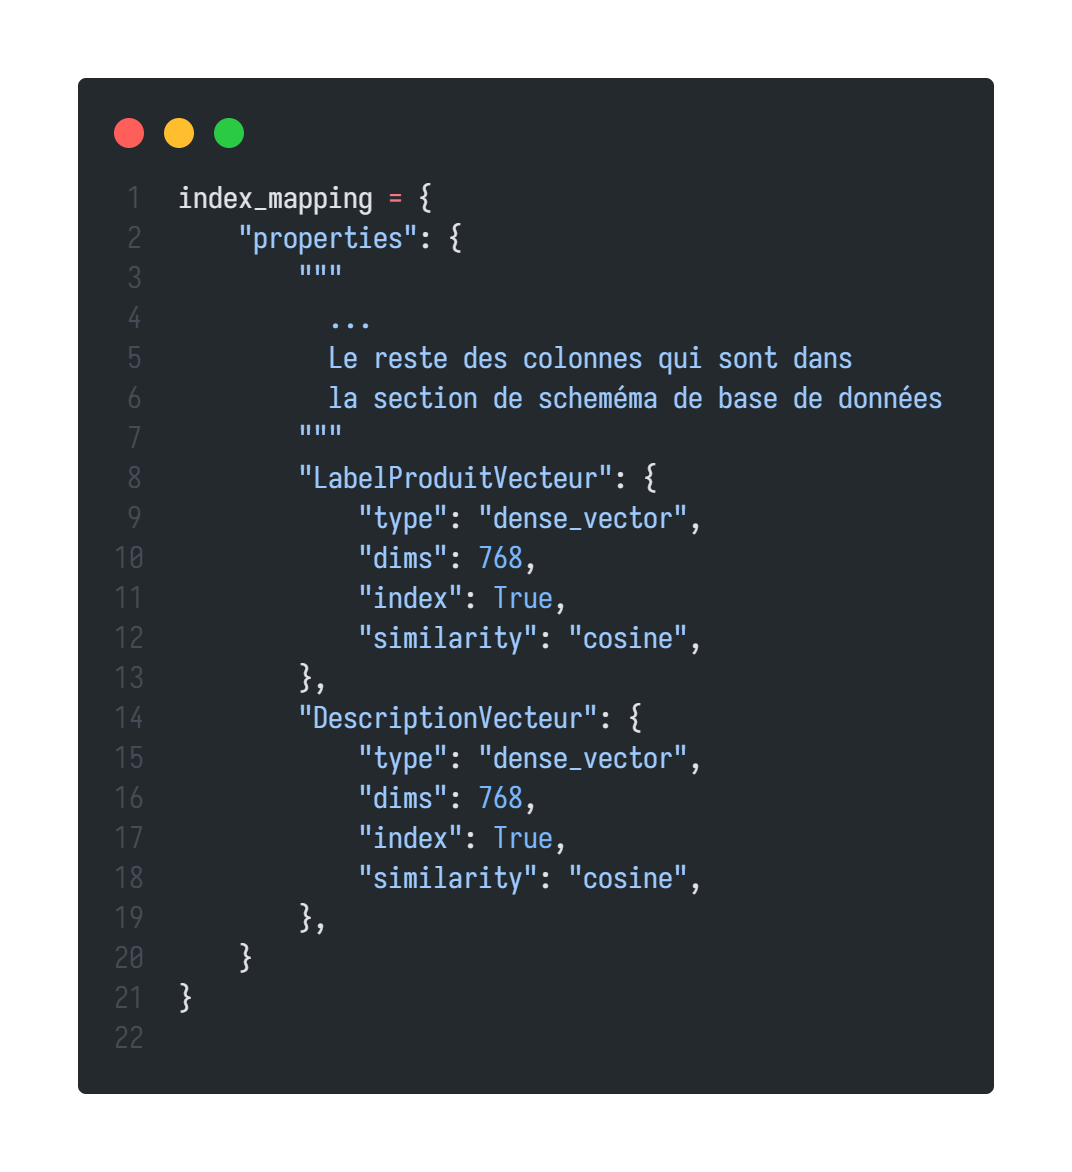
\includegraphics[width=\textwidth,height=0.75\textheight,keepaspectratio]{logos/index_mapping.png}
	\caption{Code d'index de Produit}
	\label{fig:indexmappingproduit}
\end{figure}

\newpage
\noindent
On commence par la création d'un objet << index\_mapping >> qui contient un objet << propriétés >> contenant toutes les colonnes de l'index dans Elasticsearch, le reste des colonnes sont les mêmes que dans le tableau ~\ref{tab:produit_table}. Concentrons-nous sur les 2 dernières colonnes, qui sont les colonnes les plus importantes, les vecteurs que nous allons utiliser pour notre recherche. Les deux colonnes sont de type dense\_vector, indiquant qu'elles sont des vecteurs, la contrainte << dims >> qui a une valeur de 768, indique que ces vecteurs sont à 768 dimensions, << index >> qui a la valeur True, indique qu'ils sont indexables, c'est à dire qu'on peut utiliser cette colonne pour effectuer une comparaison du similarité, qui est de type << cosine >> qui indique que Elasticsearch va effectuer une similarité cosinus, qu'on va expliquer en plus de détails dans les sections suivantes.

\subsection{Le modéle Sentence-Transformers et encodage des phrases}
\noindent
Comme on a mentionné, le modéle Sentence-Transformers qu'on va utiliser est << all-mpnet-base-v2 >>, qu on l'importe de cette façon:

\begin{figure}[H]
	\centering
	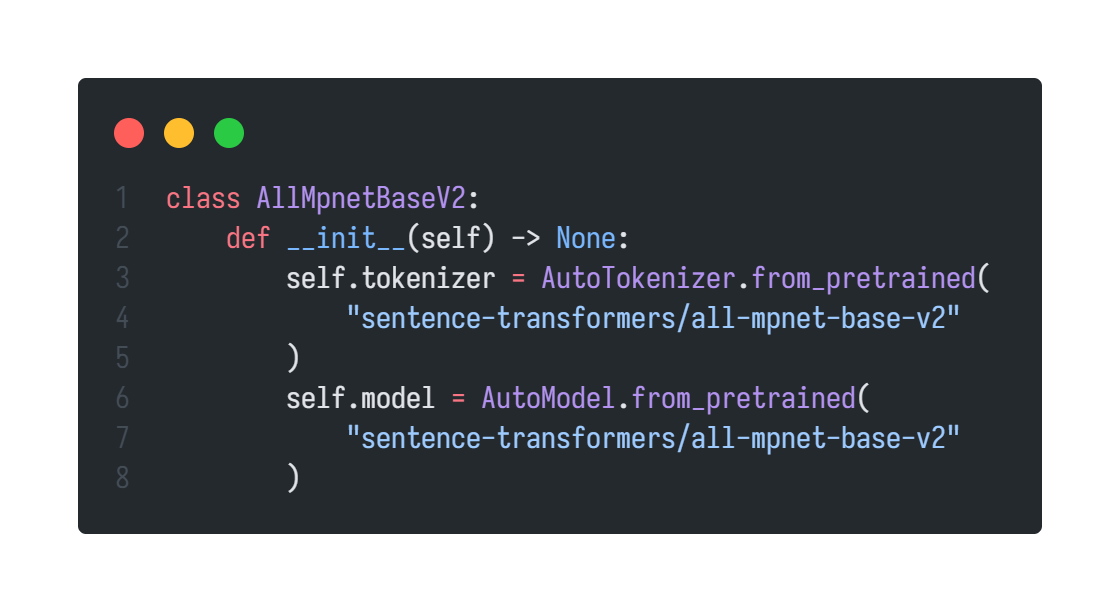
\includegraphics[width=\textwidth,height=0.75\textheight,keepaspectratio]{logos/import_model.png}
	\caption{Code d'importation de modéle Sentence-Transformers}
	\label{fig:importmodel}
\end{figure}

\newpage
\noindent
On utilise AutoTokenizer pour importer le Tokeniser du modéle, aussi que AutoModel pour importer le modèle. Le modéle est besoin d'un << Tokenizer >> puisqu'il ne peux pas comprendre du texte, on doit convertir chaque phrase en une représentation numérique. Le processus est appelé la << tokenisation >> qui est le processus de conversion d'une séquence de caractères en une séquence de jetons(tokens), ce token représente généralement un mot, il y'a aussi des tokens comme le token << CLS >> qui est le << Classify Token >>, il est mis au debut, pour marquer que c'est une phrase, et le token << PAD >>, qui es utilisé quand il y a plusieurs phrases a tokeniser, et pour ça, il est besoin de rendre toutes les phrases de même longueur. Le token << CLS >> à un identifiant de 101, et << PAD >> à un identifiant de 0. La figure ~\ref{fig:tokenisationexp} illustre un exemple simple de Tokenisation.

\begin{figure}[H]
	\centering
	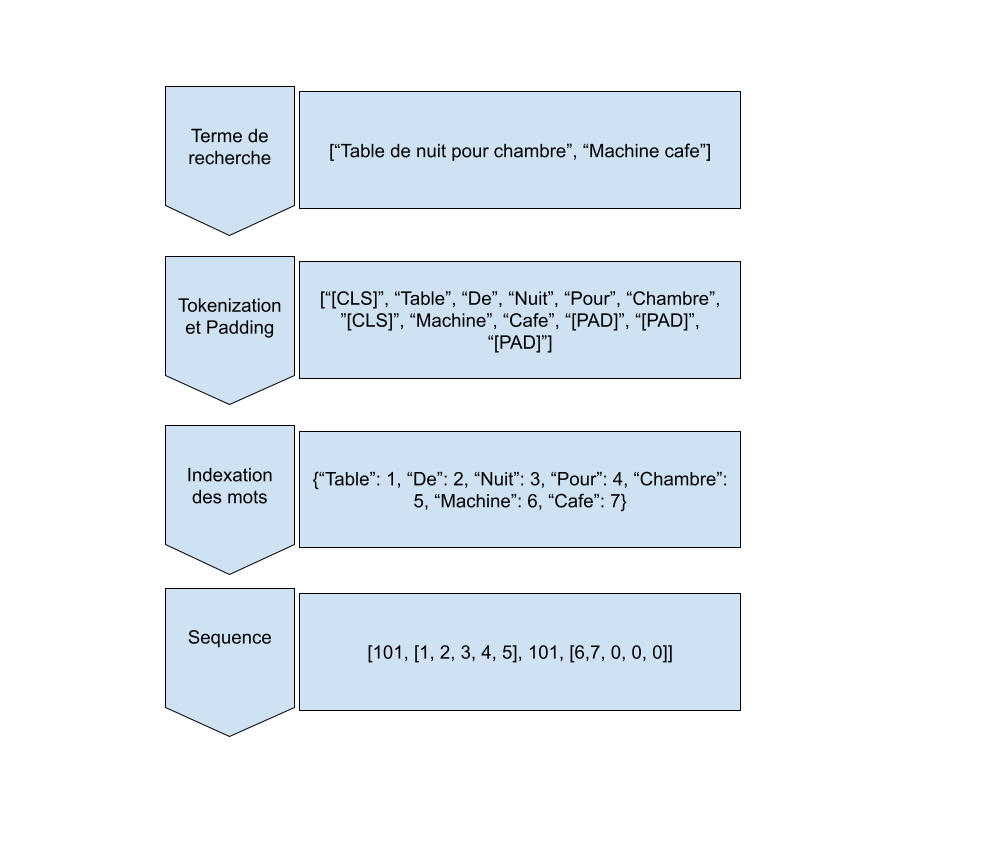
\includegraphics[width=0.9\textwidth]{logos/tokenisation.png}
	\caption{Exemple de processus de Tokenisation}
	\label{fig:tokenisationexp}
\end{figure}

\subsubsection{Comment le modèle encode une phrase?}
\noindent
On a crée une méthode appelé "encode\_sentence\_and\_normalise" pour faire l'encodage en faisant les étapes mentionné dans la partie précédente en ajoutant une autre étape qui est trés importante, qui est le Mean Pooling. \\
D'abord, on utilise le tokeniser pour effectuer la tokenisation et le padding sur la phrase, en a effectué << truncation >> a True au cas où la phrase dépasse la limite des mots par phrase pour notre modéle qui est 368 mots, il va seulement prendre les 368 premiéres mots si la phrase dépasse la limite. Ensuite, on utilise la méthode << no\_grad >> de Pytorch, pour désactiver les << Gradients >> et passer les séquences tokenisés au modéle pour faire l'encodage.

\newpage
\subsubsection{Que'est ce qu'un << Gradient >>?}
\noindent
Un gradient consiste à mettre à jour les poids de chaque neurone de la dernière couche vers la première. Il vise à corriger les erreurs selon l'importance de la contribution de chaque élément à celles-ci. Mais dans notre cas, on dèsactive les calculs des << gradients >> pour un nombre des raisons importantes qui sont citès dans \citetitle{pytorch:nograd} (\cite{pytorch:nograd}), tels que:

\begin{enumerate}
	\item \small\textbf{Contrôle du calcul du gradient: }Dans notre cas, le modèle est utilisé pour l'inférence, c'est-à-dire pour générer des vecteurs pour une phrase d'entrée donnée. Puisqu'il n'est pas nécessaire de calculer les gradients pendant l'inférence, l'utilisation de torch.no\_grad() évite une consommation inutile de mémoire et une surcharge de calcul en désactivant le suivi des gradients.
	\item \small\textbf{Optimisation de la mémoire: }Lors de l'inférence, il n'est pas nécessaire de calculer les gradients car les paramètres du modèle ne sont pas mis à jour. En désactivant le calcul du gradient, nous économisons de la mémoire qui serait autrement utilisée pour stocker les informations sur le dégradé. Cela peut être particulièrement important pour les grands modèles ou lorsqu’il s’agit de longues séquences.

	\item \small\textbf{Optimisation de la vitesse: }La désactivation du calcul du gradient accélère également le processus, car le framework n'a pas besoin d'effectuer les calculs supplémentaires requis pour le suivi du gradient.
\end{enumerate}

\noindent
Après que le modéle fais l'encodage de phrase, il nous donne un output qui consiste de plusieurs vecteurs qui représente chaque mot de la phrase. De coup, on a plusieurs vecteurs, c'est à dire chaque mot est isolée, donc on est besoin d'une méthode pour regrouper ces mots, et prendre le contexte de toute la phrase, c'est là qu'intervient la méthode de << Mean Pooling >>.

\newpage
\subsubsection{Le Mean Pooling}
\noindent
Le Mean Pooling est un processus qui calcule efficacement la moyenne de la sequence obtenu aprés le padding et la tokenisation tout en ignorant les jetons de remplissage (padding tokens) qui ont une valeur de 0, ce qui donne un seul vecteur qui représente la phrase entière. La figure ~\ref{fig:meanpoolingex} illustre un exemple.

\begin{figure}[H]
	\centering
	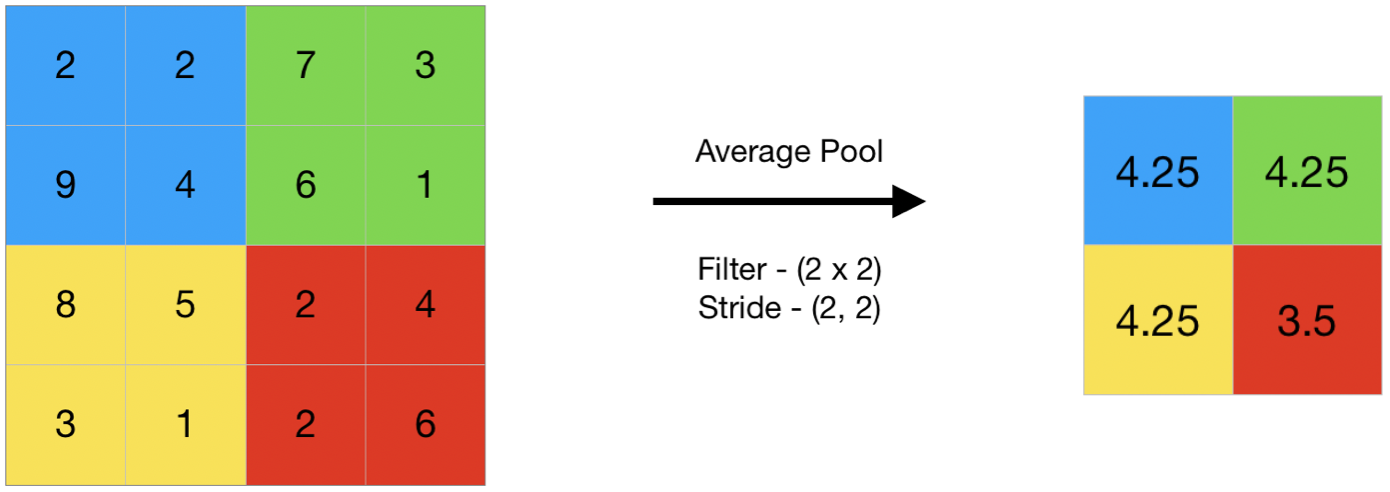
\includegraphics[width=0.9\textwidth]{logos/mean_pooling.png}
	\caption{Exemple de Mean Pooling}
	\label{fig:meanpoolingex}
\end{figure}

\noindent
Nous prenons la moyenne de chaque vecteur et on le mettons dans un seul vecteur. La figure ~\ref{fig:meanpoolingmethod} présente le code nécessaire pour cette methode.

\begin{figure}[H]
	\centering
	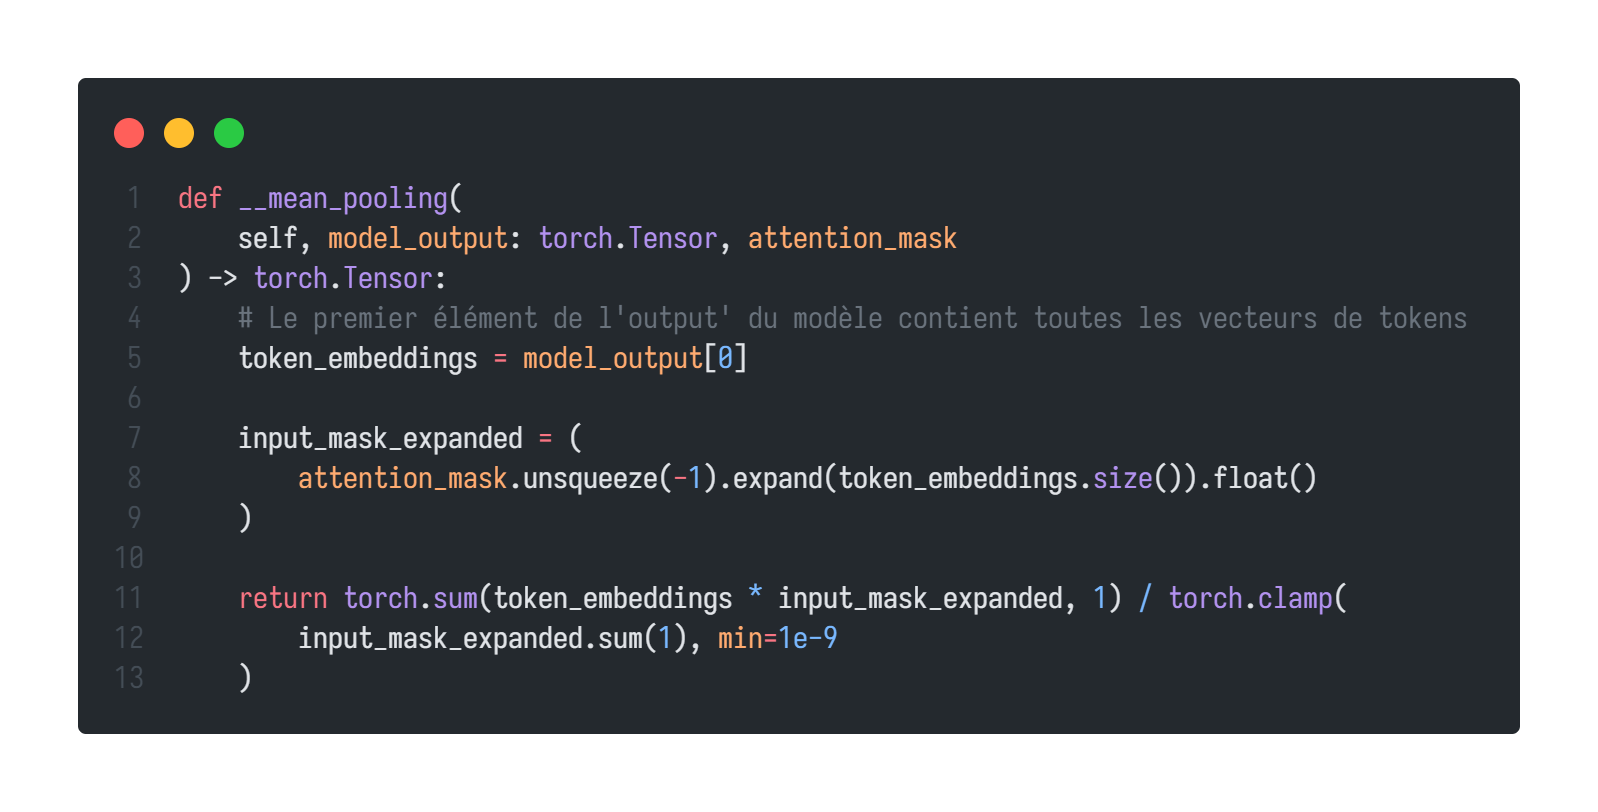
\includegraphics[width=0.9\textwidth]{logos/mean_pooling_method.png}
	\caption{Code de méthode mean\_pooling}
	\label{fig:meanpoolingmethod}
\end{figure}

\noindent
Cette méthode consiste de trois étapes, qui sont:
\begin{enumerate}
	\item \small\textbf{L'éxtraction des vecteurs des tokens: }token\_embeddings = model\_output[0] : cette ligne récupère les vecteurs de tokens à partir de l'output du modèle. Généralement, pour les modèles de Sentence-Transformers, le premier élément de la sortie (model\_output[0]) contient les intégrations de tous les tokens de la séquence d'entrée.

	\item \small\textbf{Extension du masque d'attention: }input\_mask\_expanded = \\ attention\_mask.unsqueeze(-1).expand(token\_embeddings.size()).float() : \\ Cette ligne traite le attention\_mask. Le masque d'attention est simplement un masque qui fait la différence entre le contenu et les jetons de remplissage.
	
	\begin{itemize}
		\item unsqueeze(-1) ajoute une dimension supplémentaire à la fin du attention\_mask, le rendant compatible en dimensions avec token\_embeddings lorsque nous appliquons expand().
		\item expand(token\_embeddings.size()) ajuste le masque pour qu'il corresponde aux dimensions de token\_embeddings, répétant efficacement le masque pour chaque dimension vecteur.
		\item .float() convertit le masque en float, facilitant les opérations mathématiques ultérieures avec token\_embeddings.
	\end{itemize}

	\item \small\textbf{Application du masque et calcul de Mean Pooling: }
	\begin{itemize}
		\item torch.sum(token\_embeddings * input\_mask\_expanded, 1) : ceci calcule la somme des vecteurs dans la dimension de séquence (dimension 1), mais uniquement pour les vecteurs correspondant aux jetons de données réels (pas de padding(0)), comme indiqué par input\_mask\_expanded.
		\item torch.clamp(input\_mask\_expanded.sum(1), min=1e-9) : La somme des vecteurs est ensuite divisée par la somme de input\_mask\_expanded le long de la dimension de séquence, ce qui donne le nombre de tokens sans padding. torch.clamp garantit que nous ne divisons pas par zéro en définissant une valeur minimale (1e-9), empêchant ainsi les erreurs de division par zéro.
	\end{itemize}
\end{enumerate}
\newpage
\noindent
La figure ~\ref{fig:encodesentence} illustre la méthode compléte pour l'encodage d'une phrase.

\begin{figure}[H]
	\centering
	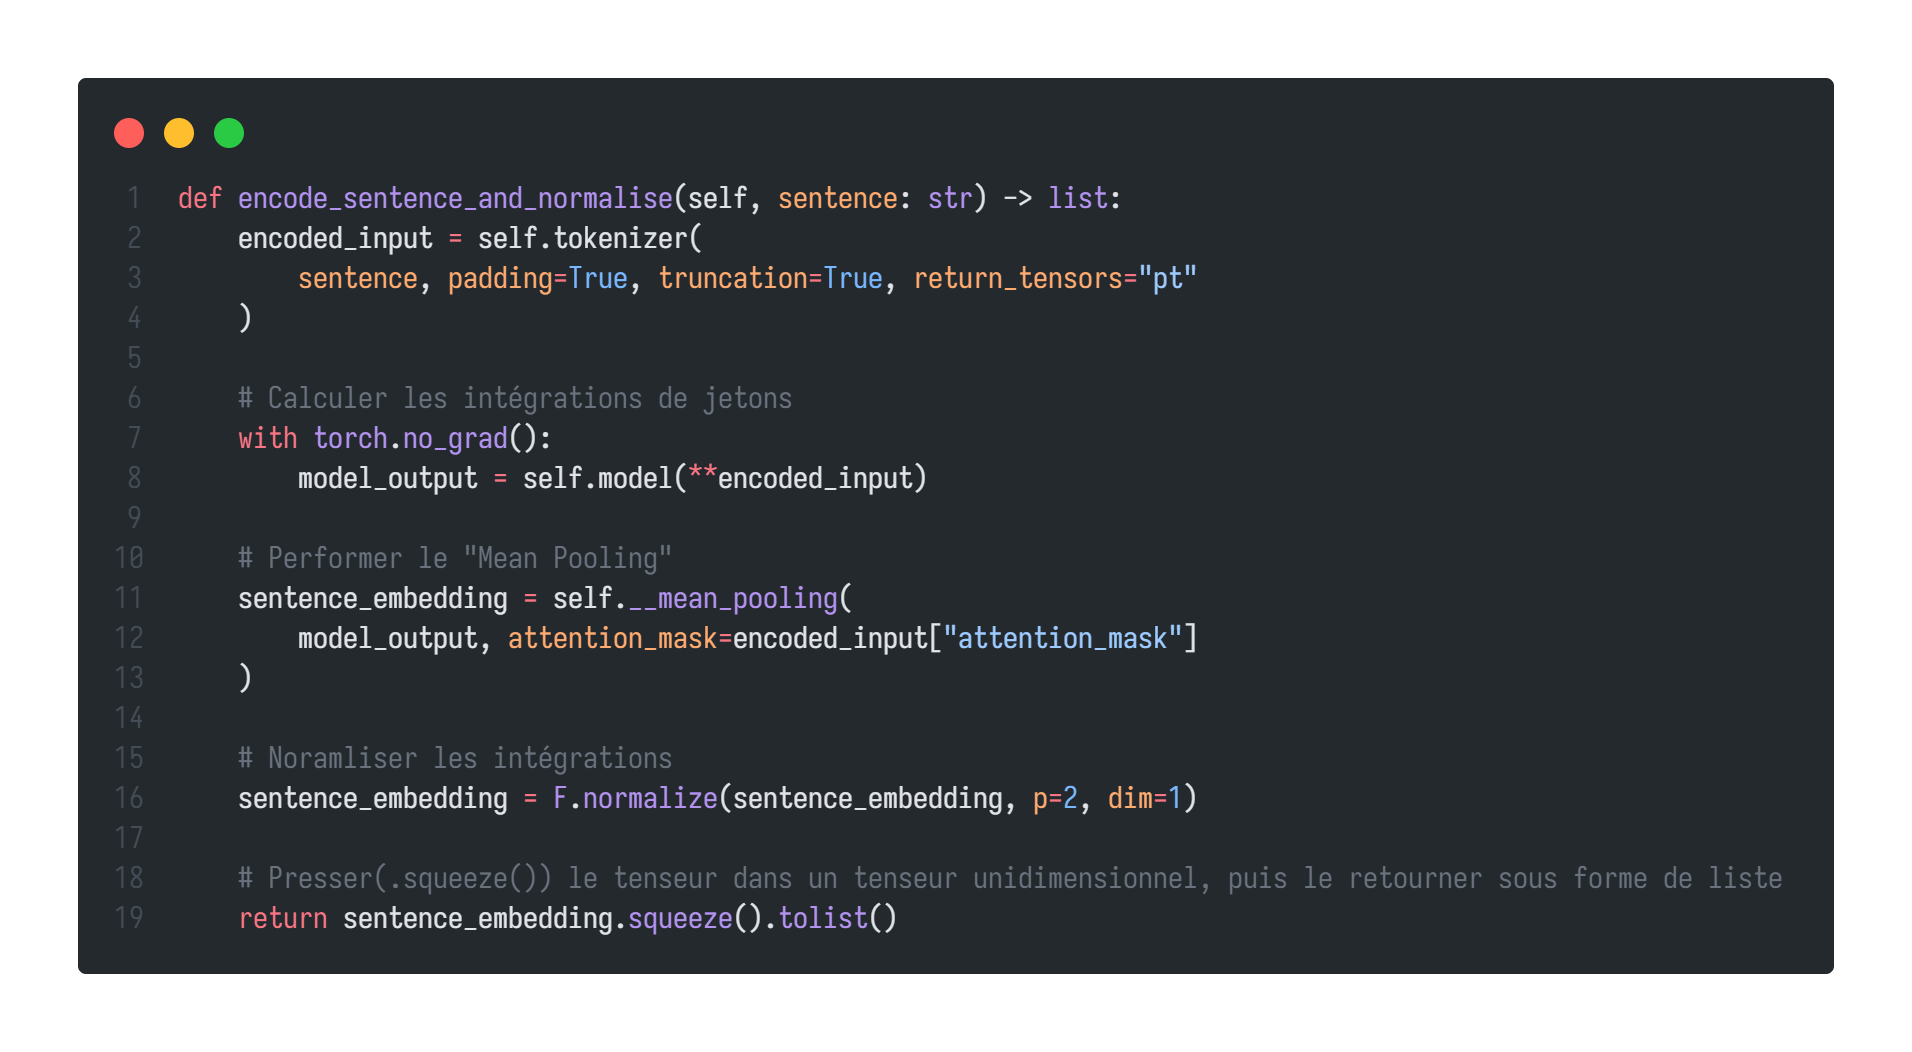
\includegraphics[width=\textwidth]{logos/encode_sentence.png}
	\caption{Méthode encode\_sentence\_and\_normalise}
	\label{fig:encodesentence}
\end{figure}

\subsection{Elasticsearch et utilisation de la similarité cosinus dans le recherche vectorielle}
\noindent
Pour effectuer notre méthode de recherche qui est le recherche vectorielle, il faut d'abord ajouter les vecteurs avec lesquels nous voulons comparer, et les ajouter dans notre base de données qui est Elasticsearch. Pour effectuer ça, on va utiliser la méthode qu'on a crée << encode\_sentence\_and\_normalise >> pour générer les vecteurs, mais d'abord, on doit créer une instance de notre modéle, on a appelé cette classe AllMpnetBaseV2. Dans notre cas on veux utiliser les colonnes << Bréve Description >> et << SEO Label Produit >>, donc on va faire l'encodage pour chaque ligne dans deux nouveaux colonnes << DescriptionVecteur >> et << LabelProduitVecteur >>. \\ La figure ~\ref{fig:encoding} montre le code pour cette étape.

\begin{figure}[H]
	\centering
	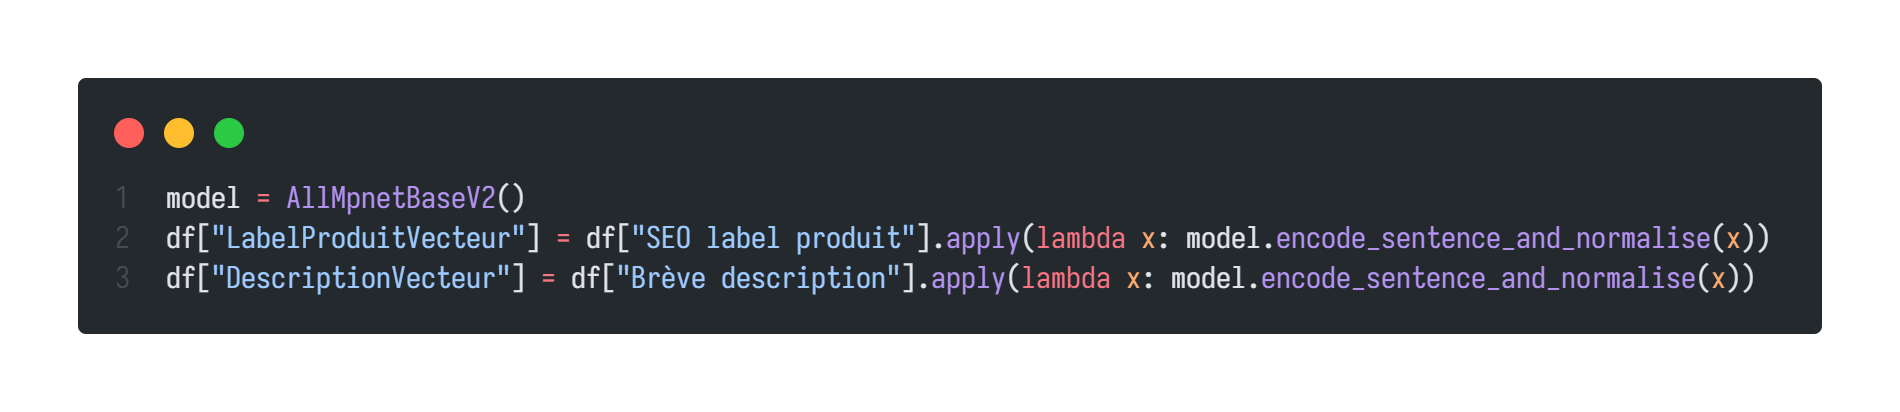
\includegraphics[width=\textwidth]{logos/vectors.png}
	\caption{Encodage des deux colonnes Bréve Déscription et SEO Label Produit}
	\label{fig:encoding}
\end{figure}

\noindent
Le résultat de cette étape c'est qu'on obtient 2 nouvelles colonnes, << DescriptionVecteur >> et << LabelProduitVecteur >> qui sont montré dans la figure ~\ref{fig:encodedvectors}.

\begin{figure}[h]
	\centering
	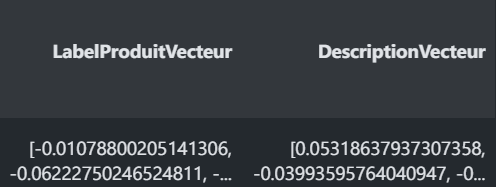
\includegraphics[width=\textwidth]{logos/encodedvectors.png}
	\caption{les deux nouvelles colonnes << descriptionvecteur >> et << labelproduitvecteur >> }
	\label{fig:encodedvectors}
\end{figure}

\noindent
L'étape suivante consiste de faire une connexion à Elasticsearch, et insérer la les données des produits. D'abord on établit une connexion à notre cluster Elasticsearch qu'on a lancé à partir de Docker, en créant une instance de class Elasticsearch et spécifiant le host, et le basic auth qui consiste de nom utilisateur et mot de passe généré par Kibana. Ensuite, nous créons notre index Elasticsearch en spécifiant notre index\_mapping qu'on a mentionné au debut de ce chapitre à travers la méthode << es.indices.create >> qui prends deux paramètres, le nom de l'index et son mapping. Enfin, nous convertissons notre CSV en object Python à travers la méthode << to\_dict >> et nous insérons chaque ligne dans Elasticsearch à travers la méthode << index >>, qui prends trois paramètres << index >>, << document >> et << id >>. \\
La figure ~\ref{fig:insertintoelastic} montre le code nécessaire pour cette étape.

\begin{figure}[h]
	\centering
	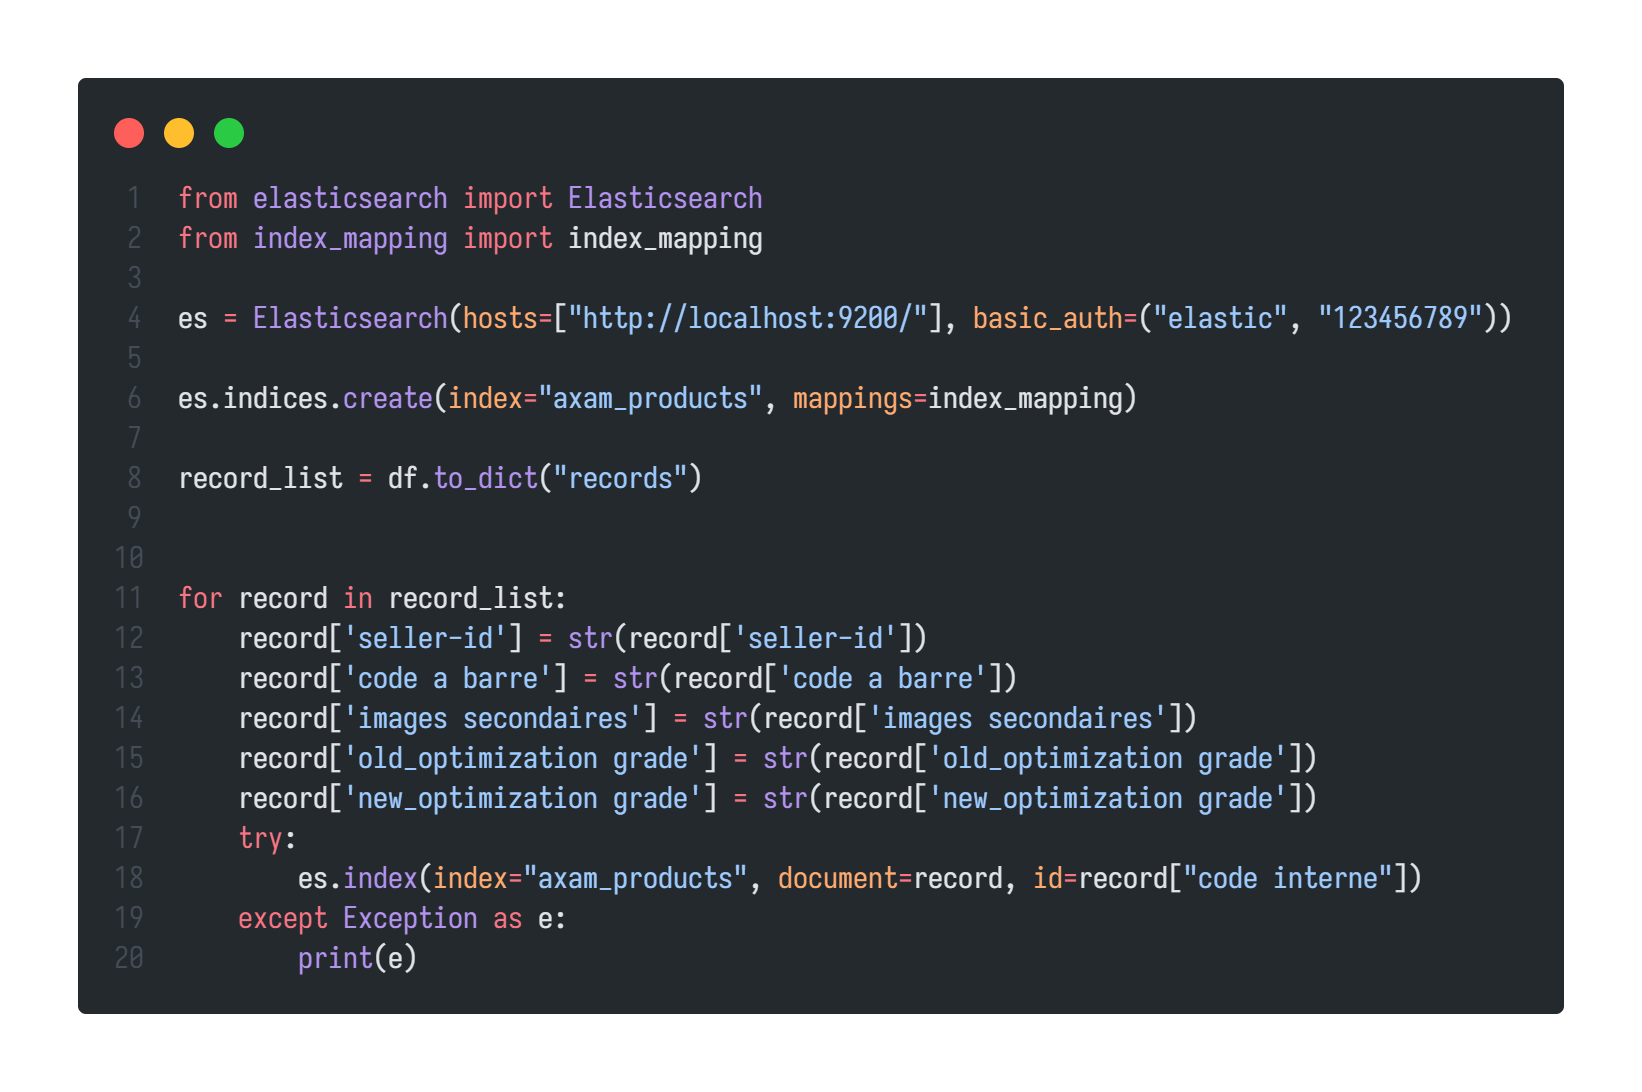
\includegraphics[width=\textwidth]{logos/insert_into_elastic.png}
	\caption{Insértion des données dans Elasticsearch}
	\label{fig:insertintoelastic}
\end{figure}